\section{Regressione Logistica con tutte le feature}
La prima tecnica implementata per la classificazione binaria è la \textit{Regressione Logistica}.\\
Come accennato nei capitoli precedenti, l'obiettivo è quello di creare un modello in grado di riconoscere quando un immagine rappresenta un tumore al cervello oppure no con le migliori prestazioni possibili.\\
L'obiettivo di tale tecnica è quella di trovare il \textit{decision boundary} che suddivida nel modo più corretto possibile i target nella classe positiva (1 = è un tumore) e nella classe negativa (0 = non è un tumore).\\
Il primo passo, oltre a quello di leggere il file csv fixato e convertirlo in dataset con Pandas, è quello di portare tutti i dati nella stessa scala di valori. Ciò è utile perchè si hanno dei range di valori molto diversi e l'algoritmo potrebbe dare più importanza ai dati con range più grande. Per questo motivo si è utilizzata la classe di scikit-learn \textit{StandardScaler}. Tale classe permette semplicemente di standardizzare il dataset, ovvero portare tutti i dati in una distribuzione con media 0 e varianza 1. Perciò applicando il modello StandardScaler sui dati si ottiene un dataset con tutti i dati nella stessa scala.\\
Dal dataset occorre estrarre i \textit{regressori} (matrice X) e i \textit{target} (vettore Y). La standardizzazione ovviamente viene applicata alla matrice X.\\
\begin{lstlisting}
from sklearn.preprocessing import StandardScaler
from sklearn.model_selection import train_test_split

X = brain_tumor_data.drop("Target", axis=1).values
Y = brain_tumor_data["Target"].values
ss = StandardScaler()
X = ss.fit_transform(X)

X_train, X_test, Y_train, Y_test = train_test_split(X, Y, test_size=0.3)
\end{lstlisting}
Per la validazione del modello si sa che è necessario avere dei dati per il \textit{training} del modello e per il test. Si è ricorso quindi al metodo \textit{train\_test\_split} di scikit-learn che applica tale divisione. Si è scelto di utilizzare il 70\% dei dati per la fase di training e il 30\% per la fase di test.\\
\begin{figure}[h]
	\centering   	
	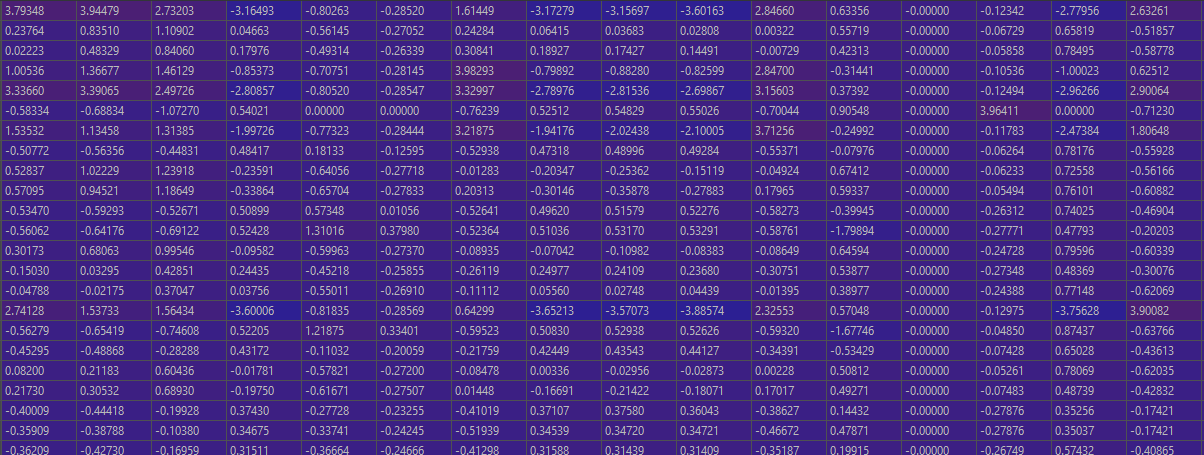
\includegraphics[width=140mm]{image/standardX.png}
	\caption{una parte della matrice X standardizzata}
\end{figure}
A questo punto si costruisce il modello di Regressione Logistica. Per farlo si utilizza la classe \textit{LogisticRegression} di scikit-learn.
\begin{lstlisting}
from sklearn.linear_model import LogisticRegression
from sklearn.metrics import accuracy_score, log_loss

log_reg = LogisticRegression()
log_reg.fit(X_train, Y_train)
Y_pred = log_reg.predict(X_test)
Y_pred_prob = log_reg.predict_proba(X_test)

acc = accuracy_score(Y_test, Y_pred)
log_loss_score = log_loss(Y_test, Y_pred_prob)
\end{lstlisting}
Con il metodo \text{fit()} di LogisticRegression si esegue la fase di training e, ovviamente, in input al metodo si passano i dati di train generati dal metodo \textit{train\_test\_split}.\\
Per valutare la bontà del modello si calcolano l' \textit{accuracy} (o accuratezza) e la \textit{Negative Log-likelihood} (o \textit{log loss}). L'accuracy è un indice che va da 0 a 1 che conta quante classificazioni son state fatte correttamente, mentre la log loss tiene conto della probabilità di appartenenza ad una determinata classe. Si punta ad avere un accuracy più alta possibile e una log loss più bassa possibile.

\section{Regressione Logistica con Dimensionality Reduction}
Il dataset è formato da 17 feature. Può essere una buona mossa applicare una tecnica di Dimensionality Reduction per poi fare classificazione? \\
Per capirlo si è utilizzata la tecnica \textit{PCA} in 2D, 3D e di dimensione tale da spiegare almeno il 95\% di varianza dei dati.
\begin{lstlisting}
from sklearn.decomposition import PCA

pca = PCA(n_components=2)
principal_components = pca.fit_transform(X)
principalDF = pd.DataFrame(data=principal_components,
columns=['principal component 1', 'principal component 2'])

finalDf = pd.concat([principalDF, brain_tumor_data[['Target']]], axis=1)

X = finalDf.drop("Target", axis=1)
Y = finalDf["Target"].values

X_train, X_test, Y_train, Y_test = train_test_split(X, Y, test_size=0.3)
\end{lstlisting}
Si è utilizzata la classe \textit{PCA} di scikit-learn. Tale classe, applicando il metodo \textit{fit\_transform()} sulla matrice X, seleziona le componenti principali (2 nel caso di PCA 2D e 3 nel caso di PCA 3D) in una matrice. Per utilizzare i dati nella tecnica di Regressione Logistica è necessario averli in formato dataframe, perciò mediante i metodi di Pandas \textit{DataFrame()} e \textit{concat()} si è costruito il nuovo dataframe con le sole componenti principali. Dopodiché si suddividono i dati di training e di test e si applica la Regressione Logistica nello stesso modo in cui è stato applicato nella sezione precedente.\\
Uno degli scopi della tecnica PCA è quella della \textit{Data Visualization}. Infatti per le tecniche di PCA in 2D e 3D vi sono porzioni di codice per la proiezione dei dati in 2D e 3D.
Per la rappresentazione in 2D è sufficiente costruire uno scatter dove negli assi vi sono le due componenti principali. I target rappresentati possono essere rossi se il valore è 1 (cioè è un tumore) e verdi se il valore è 0 (non è un tumore).
\newpage
\begin{lstlisting}
fig = plt.figure(figsize=(8, 8))
ax = fig.add_subplot(1, 1, 1)
ax.set_xlabel('Principal Component 1', fontsize=15)
ax.set_ylabel('Principal Component 2', fontsize=15)
ax.set_title('2 Component PCA', fontsize=20)


targets = [1, 0]
colors = ['r', 'g']
for target, color in zip(targets, colors):
indicesToKeep = finalDf['Target'] == target
ax.scatter(finalDf.loc[indicesToKeep, 'principal component 1']
, finalDf.loc[indicesToKeep, 'principal component 2']
, c=color
, s=50)
ax.legend(targets)
ax.grid()
plt.show()
\end{lstlisting}
Il risultato è il seguente:\\
\begin{figure}[h]
	\centering   	
	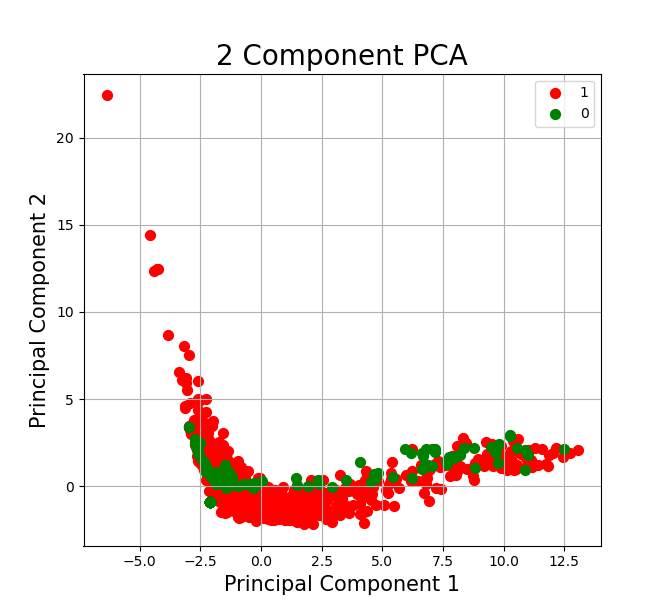
\includegraphics[width=100mm]{image/scatter2d.png}
\end{figure}
\\Per quanto riguarda la Data Visualization in 3D si utilizza la classe \textit{Axes3D} del modulo \textit{mpl\_toolkits}. La classe Axes3D permette di costruire un diagramma cartesiano con tre assi. Sui tre assi si hanno le tre componenti principali.\\
L'idea di base è quella di costruire uno scatter (come nel caso precedente) di tre dimensioni mediante matplotlib e passarlo in input alla classe Axes3D che permette la rappresentazione cartesiana.
\begin{lstlisting}
from mpl_toolkits.mplot3d import Axes3D

fig = plt.figure()
finalDf['Target'] = pd.Categorical(finalDf['Target'])
my_color = finalDf['Target'].cat.codes
ax = Axes3D(fig)
ax.scatter(finalDf['PCA1'], finalDf['PCA2'], finalDf['PCA3'], c=my_color, cmap="Set2_r", s=60)

xAxisLine = ((min(finalDf['PCA1']), max(finalDf['PCA1'])), (0, 0), (0, 0))
ax.plot(xAxisLine[0], xAxisLine[1], xAxisLine[2], 'r')
yAxisLine = ((0, 0), (min(finalDf['PCA2']), max(finalDf['PCA2'])), (0, 0))
ax.plot(yAxisLine[0], yAxisLine[1], yAxisLine[2], 'r')
zAxisLine = ((0, 0), (0, 0), (min(finalDf['PCA3']), max(finalDf['PCA3'])))
ax.plot(zAxisLine[0], zAxisLine[1], zAxisLine[2], 'r')

ax.set_xlabel("PC1")
ax.set_ylabel("PC2")
ax.set_zlabel("PC3")
ax.set_title("PCA on the iris data set")
plt.show()
\end{lstlisting}
Il risultato è il seguente:\\
\begin{figure}[h]
	\centering   	
	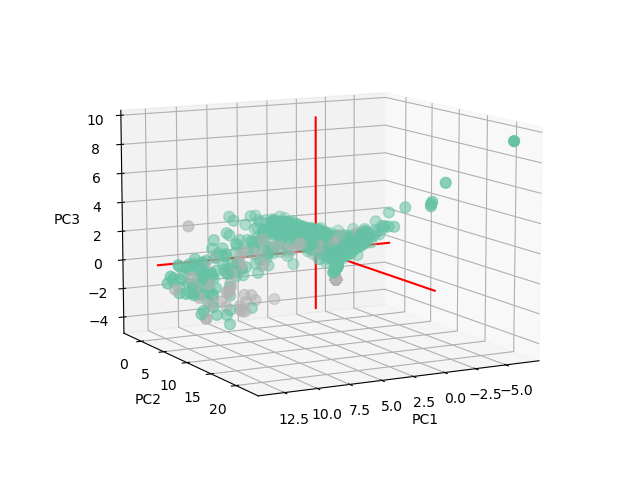
\includegraphics[width=100mm]{image/grafico3d.png}
\end{figure}

\section{Conclusione sulla Regressione Logistica}
La regressione logistica utilizzando tutte le feature è quella che dà i risultati migliori, sia in termini di accuracy e di log loss.\\
Per quanto riguarda l'utilizzo della tecnica PCA, il risultato migliore è dato dalla PCA con parametro il 95\% di varianza spiegata. In particolare, applicando dimensionality reduction a due dimensioni con PCA 2D ha peggiorato le prestazioni del modello. Ciò era intuibile guardando il grafico in due dimensioni, dove è difficile trovare un decision boundary lineare che suddivida la classe negativa con quella positiva. La situazione migliora di molto nel caso di PCA 3D, dove le prestazioni sono di poco peggiori a quelle di Regressione Logistica con PCA 95\%.
\begin{figure}[h]
	\centering   	
	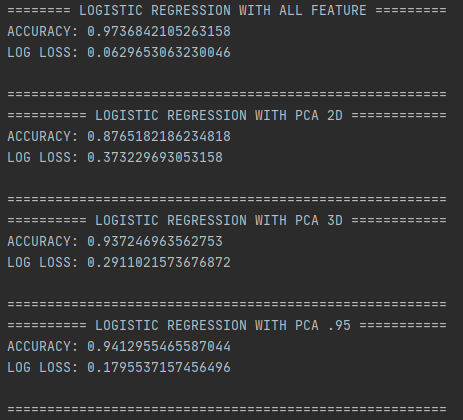
\includegraphics[width=60mm]{image/regressionelogisticaresults.png}
	\caption{Visualizzazione dei risultati stampati sulla console Python.}
\end{figure}